% Options for packages loaded elsewhere
\PassOptionsToPackage{unicode}{hyperref}
\PassOptionsToPackage{hyphens}{url}
\documentclass[
  ignorenonframetext,
]{beamer}
\newif\ifbibliography
\usepackage{pgfpages}
\setbeamertemplate{caption}[numbered]
\setbeamertemplate{caption label separator}{: }
\setbeamercolor{caption name}{fg=normal text.fg}
\beamertemplatenavigationsymbolsempty
% remove section numbering
\setbeamertemplate{part page}{
  \centering
  \begin{beamercolorbox}[sep=16pt,center]{part title}
    \usebeamerfont{part title}\insertpart\par
  \end{beamercolorbox}
}
\setbeamertemplate{section page}{
  \centering
  \begin{beamercolorbox}[sep=12pt,center]{section title}
    \usebeamerfont{section title}\insertsection\par
  \end{beamercolorbox}
}
\setbeamertemplate{subsection page}{
  \centering
  \begin{beamercolorbox}[sep=8pt,center]{subsection title}
    \usebeamerfont{subsection title}\insertsubsection\par
  \end{beamercolorbox}
}
% Prevent slide breaks in the middle of a paragraph
\widowpenalties 1 10000
\raggedbottom
\AtBeginPart{
  \frame{\partpage}
}
\AtBeginSection{
  \ifbibliography
  \else
    \frame{\sectionpage}
  \fi
}
\AtBeginSubsection{
  \frame{\subsectionpage}
}
\usepackage{iftex}
\ifPDFTeX
  \usepackage[T1]{fontenc}
  \usepackage[utf8]{inputenc}
  \usepackage{textcomp} % provide euro and other symbols
\else % if luatex or xetex
  \usepackage{unicode-math} % this also loads fontspec
  \defaultfontfeatures{Scale=MatchLowercase}
  \defaultfontfeatures[\rmfamily]{Ligatures=TeX,Scale=1}
\fi
\usepackage{lmodern}
\ifPDFTeX\else
  % xetex/luatex font selection
\fi
% Use upquote if available, for straight quotes in verbatim environments
\IfFileExists{upquote.sty}{\usepackage{upquote}}{}
\IfFileExists{microtype.sty}{% use microtype if available
  \usepackage[]{microtype}
  \UseMicrotypeSet[protrusion]{basicmath} % disable protrusion for tt fonts
}{}
\makeatletter
\@ifundefined{KOMAClassName}{% if non-KOMA class
  \IfFileExists{parskip.sty}{%
    \usepackage{parskip}
  }{% else
    \setlength{\parindent}{0pt}
    \setlength{\parskip}{6pt plus 2pt minus 1pt}}
}{% if KOMA class
  \KOMAoptions{parskip=half}}
\makeatother
\usepackage{longtable,booktabs,array}
\newcounter{none} % for unnumbered tables
\usepackage{calc} % for calculating minipage widths
\usepackage{caption}
% Make caption package work with longtable
\makeatletter
\def\fnum@table{\tablename~\thetable}
\makeatother
\usepackage{graphicx}
\makeatletter
\newsavebox\pandoc@box
\newcommand*\pandocbounded[1]{% scales image to fit in text height/width
  \sbox\pandoc@box{#1}%
  \Gscale@div\@tempa{\textheight}{\dimexpr\ht\pandoc@box+\dp\pandoc@box\relax}%
  \Gscale@div\@tempb{\linewidth}{\wd\pandoc@box}%
  \ifdim\@tempb\p@<\@tempa\p@\let\@tempa\@tempb\fi% select the smaller of both
  \ifdim\@tempa\p@<\p@\scalebox{\@tempa}{\usebox\pandoc@box}%
  \else\usebox{\pandoc@box}%
  \fi%
}
% Set default figure placement to htbp
\def\fps@figure{htbp}
\makeatother
\setlength{\emergencystretch}{3em} % prevent overfull lines
\providecommand{\tightlist}{%
  \setlength{\itemsep}{0pt}\setlength{\parskip}{0pt}}
% Auto-generated by infrastructure/rendering/_pdf_latex_helpers.py::extract_math_font_preamble.
% Minimal header passed to Pandoc via -H so Beamer slides pick up the same math font
% as the combined-PDF path. Adjust the manuscript's preamble.md to change the font globally.
\usepackage{unicode-math}
\setmathfont{latinmodern-math.otf}

% Slide layout defaults for warning-clean scientific decks.
\usepackage{etoolbox}
\IfFileExists{xurl.sty}{\usepackage{xurl}}{}
\IfFileExists{seqsplit.sty}{\usepackage{seqsplit}}{\newcommand{\seqsplit}[1]{#1}}
\protected\def\breakseq#1{\seqsplit{#1}}
\protected\def\breaktt#1{\begingroup\ttfamily\seqsplit{#1}\endgroup}
\setlength{\emergencystretch}{6em}
\tolerance=5000
\hbadness=10000
\hfuzz=1pt
\setlength{\tabcolsep}{2pt}
\AtBeginEnvironment{longtable}{\tiny\renewcommand{\arraystretch}{0.86}\setlength{\tabcolsep}{1pt}}
\AtBeginEnvironment{tabular}{\tiny\renewcommand{\arraystretch}{0.86}\setlength{\tabcolsep}{1pt}}

% Natbib and cross-reference fallbacks — slides don't load natbib
% or cleveref, but combined-PDF manuscript prose may emit these
% commands. The fallback renders citations as a bracketed key list
% and cross-references as detokenized labels so slides don't fail on
% undefined control sequences or raw underscores. \providecommand is
% a no-op if packages load later.
\providecommand{\citep}[1]{[#1]}
\providecommand{\citet}[1]{#1}
\providecommand{\citealp}[1]{#1}
\providecommand{\citeauthor}[1]{#1}
\providecommand{\citeyear}[1]{#1}
\providecommand{\cref}[1]{\texttt{\detokenize{#1}}}
\providecommand{\Cref}[1]{\texttt{\detokenize{#1}}}
\usepackage{bookmark}
\IfFileExists{xurl.sty}{\usepackage{xurl}}{} % add URL line breaks if available
\urlstyle{same}
% fallback for those not using the hyperref driver hyperxmp:
\makeatletter
\@ifundefined{xmpquote}{\newcommand{\xmpquote}[1]{#1}}{}
\makeatother
\hypersetup{
  hidelinks,
  pdfcreator={LaTeX via pandoc}}

\author{\texorpdfstring{}{}}
\date{}

\begin{document}

\section{Methods: Source-Owned Token Injection and Conditional IMRAD
Assembly}\label{methods-source-owned-token-injection-and-conditional-imrad-assembly}

\begin{frame}[fragile,allowframebreaks]{Methods: Source-Owned Token
Injection and Conditional IMRAD Assembly}
The method is conditional section hydration. Each slot combines the
seed, slot name, category, ordinal, and full category list into a
SHA-256 digest; the digest indexes the configured category. Including
the full category list in the digest input means that a lexicon edit can
change the plan in a deterministic and reviewable way instead of
silently preserving stale output.

The deterministic digest recipe is deliberately narrow. It does not
sample from ambient prose, project history, or renderer state; it uses
only the committed seed, the slot declaration, the category name, the
ordinal for repeated slots, and the ordered category inventory. A fork
can therefore explain a changed token choice as a changed seed, slot, or
lexicon row rather than as an opaque generation event.

The first review scenario is declared before generation. The project
names its scope as a local exemplar, records enabled sections, keeps DOI
and publication claims blank, and treats the copy stage as a review
handoff. That ordering matters because a reader should know the allowed
claim boundary before inspecting fluent generated text.

The governing constraint is publication claims stay local until release.
The source manuscript is intentionally sparse: it contains section
titles and large-grain placeholders, not generated claims. The project
script first validates the \texttt{madlib:} block, expands slots into a
\texttt{TokenPlan}, builds section bodies, writes artifact JSON, emits a
figure registry, and only then writes hydrated Markdown under
\breaktt{output/manuscript/}.

The configured method moves are validate config before composition,
declare review scenario and method invariants, separate explicit YAML
fields from loader defaults, govern lexicon categories as reviewable
data, expand slots through seeded digest selection, allocate slot
choices to enabled manuscript sections, compose conditional section
bodies, assemble method evidence tables and visual audit figures, align
generated claims with the claim ledger, emit evidence artifacts before
rendering, verify that no unresolved placeholders remain, assemble a
reviewer packet from regenerated artifacts, and preserve human review
before publication claims. The protocol sequence is Ingest declared
manuscript schema produces \texttt{MadlibConfig}; Declare review
scenario produces \breaktt{review\ scenario}; Track field origin produces
\breaktt{explicit/default\ path\ inventory}; Govern lexicon categories
produces \breaktt{validated\ lexicon}; Construct digest selection
material produces \breaktt{digest\ input\ records}; Record selection
invariants produces \breaktt{selection\ invariant\ set}; Expand slot
declarations produces \texttt{TokenPlan}; Apply section conditions
produces \breaktt{enabled\ section\ set}; Compose conditional IMRAD
bodies produces \breaktt{section\ variables}; Assemble evidence tables
produces \breaktt{Markdown\ evidence\ tables}; Align claims with evidence
ledger produces \breaktt{claim-aligned\ evidence\ surface}; Generate
visual audit surface produces \breaktt{registered\ figure\ set}; Emit
machine-readable artifacts produces
\breaktt{output/data,\ output/reports,\ and\ output/figures}; Hydrate
manuscript shell produces \breaktt{output/manuscript}; Render and
validate deliverables produces \breaktt{validated\ project\ output};
Assemble reviewer packet produces \texttt{review\ packet}; Copy review
surface produces \breaktt{copied\ publication-review\ bundle}; Document
fork migration produces \breaktt{fork\ migration\ notes}. These steps
make the method auditable from three directions: tests inspect the
Python behavior, generated artifacts expose the token plan, and
manuscript validation confirms that no unresolved placeholder survives
into rendered outputs.

The config-origin inventory currently separates 125 explicit YAML
path(s) from 11 loader-defaulted path(s). Treating origin as method
evidence prevents a rendered field from looking equally authored when it
was actually inherited from the loader. The same inventory drives
configured-field tables and figures, so reviewers can inspect which
schema blocks were intentionally set before judging the generated prose.

Method invariants are reviewed as their own artifact. Token choices are
allowed to change when the seed, slot name, category, ordinal, or
ordered category inventory changes; they are not allowed to change
because PDF rendering, HTML rendering, file-copy order, or hand-edited
output changed. This separates generation logic from presentation logic.

Lexicon governance is handled as data governance. Required categories
must be nonempty, optional categories remain project-owned when
declared, and the selected 40 token choice(s) stay bound to 10
configured category list(s). The slot-to-section allocation is abstract:
3, authoring\_contract: 2, configuration: 1, discussion: 3, evaluation:
5, introduction: 8, limitations: 3, methods: 6, reproducibility: 2,
results: 5, scope: 2, which lets the Methods, Results, and provenance
tables state where each lexical decision enters the manuscript.

Conditional section generation is handled before prose assembly. A
disabled section does not vanish and does not borrow claims from an
enabled section; it resolves to an explicit statement that names the
controlling \breaktt{madlib.section\_conditions} key. That behavior keeps
negative or excluded material visible to reviewers.

Evidence tables and visual audit figures are generated from the same
config and \texttt{TokenPlan}. Enabled visualizations are
configured\_field\_matrix, section\_configuration\_heatmap,
field\_origin\_summary, token\_injection\_flow,
section\_token\_allocation, provenance\_trace\_map,
quality\_gate\_matrix; they summarize field origin, token density,
injection flow, section allocation, provenance, and quality gates
without adding independent claims. Figure registration is therefore a
method step: every manuscript image has to be written, registered, and
validated as part of the reproducible render path.

Claim-ledger alignment is part of composition. The contribution table
can make local method claims, but publication, empirical,
reader-quality, and domain-specific claims must either point to evidence
or remain explicit non-claims. This is why the claim ledger, audit
rules, limitations, and authoring contract are generated beside the
Methods rather than written after the fact.

Evaluation is part of the method rather than an afterthought. The config
declares quality probes (Method row completeness, Field-origin
visibility, Placeholder survival, Provenance completeness,
Section-switch observability, Figure registry coverage, Method-figure
alignment, Evidence cleanliness, Fork readiness, Copied-output parity,
Digest invariant review, Claim-ledger alignment, Review packet
completeness, Fork migration sufficiency) and failure modes (Unresolved
placeholder, Overclaimed generated prose, Config-source drift, Figure
provenance gap, Domain misuse, Method row drift, Field-origin opacity,
Visual-method mismatch, Fork without validators, Digest invariant drift,
Claim ledger omission, Review packet incompleteness, Fork migration
ambiguity); the source turns them into tables and validation checks the
rendered surface. That means methods, results, evaluation, and
limitations all share one source-owned schema instead of drifting as
independent prose.

The method is organized around design principles: Configuration owns
prose choices, Method surface is config-owned, Token choice is
deterministic, Field origin is evidence, Sections are conditional but
visible, Visual audit follows data, Generated output is disposable,
Claim boundaries travel with prose, Forks must add validators,
Invariants precede rendering, Diffs are review objects, Review packet is
a method artifact, Fork migration is part of the method. These
principles prevent the Mad Lib surface from becoming a hidden authoring
channel. They require the visible manuscript to stay downstream of
declared inputs, the generated outputs to remain disposable, and the
audit surface to be broad enough for a reviewer to reconstruct how a
sentence reached the PDF.

The operational phases are Schema intake maps
\breaktt{manuscript/config.yaml} to \texttt{MadlibConfig}; Scenario
declaration maps \texttt{MadlibConfig} to \breaktt{review\ scenario};
Field-origin inventory maps \breaktt{MadlibConfig\ and\ raw\ YAML\ keys}
to \breaktt{configured\_field\_inventory.json}; Lexicon validation maps
\breaktt{madlib.lexicon\ and\ madlib.slots} to
\breaktt{validated\ slot\ inventory}; Digest token planning maps
\texttt{MadlibConfig} to \texttt{TokenPlan}; Invariant review maps
\breaktt{TokenPlan\ and\ method\ protocol} to
\breaktt{selection\ invariant\ set}; Slot-to-section allocation maps
\texttt{TokenPlan} to \breaktt{section\ token\ counts}; Section
composition maps \breaktt{TokenPlan\ and\ narrative\ moves} to
\breaktt{manuscript\ variable\ map}; Evidence table assembly maps
\breaktt{MadlibConfig\ and\ TokenPlan} to
\breaktt{manuscript\_variables.json}; Claim-ledger alignment maps
\breaktt{MadlibConfig,\ generated\ prose,\ and\ data/claim\_ledger.yaml}
to \breaktt{claim-aligned\ evidence\ surface}; Visualization emission
maps
\breaktt{MadlibConfig,\ TokenPlan,\ and\ configured-field\ inventory} to
\breaktt{output/figures\ and\ figure\_registry.json}; Artifact emission
maps \breaktt{MadlibConfig\ and\ TokenPlan} to
\breaktt{output/data,\ output/reports,\ and\ output/figures}; Manuscript
hydration maps
\breaktt{source\ manuscript\ shells\ and\ manuscript\_variables.json} to
\breaktt{hydrated\ Markdown\ manuscript}; Render maps
\breaktt{output/manuscript} to
\breaktt{output/pdf,\ output/web,\ and\ output/slides}; Validate and copy
maps \breaktt{project\ output\ directories} to
\breaktt{output/templates/template\_madlib}; Review packet assembly maps
\breaktt{validated\ project\ output\ and\ copy\ statistics} to
\texttt{review\ packet}; Fork contract documentation maps
\breaktt{source\ docs,\ authoring\ contract,\ and\ claim\ ledger} to
\breaktt{fork\ migration\ notes}. Each phase has an explicit input,
transformation, output, and guard. This makes the pipeline explainable
at manuscript scale: a reader can follow the path from YAML declarations
to token choices, from token choices to section bodies, from section
bodies to rendered artifacts, and from rendered artifacts to validation
reports.

The reviewer packet is also a method artifact. The handoff surface is
hydrated Markdown, combined PDF, web output, slides, figures, data JSON,
reports, validation results, and copy statistics; a PDF alone is
insufficient because it cannot show the token inventory, field-origin
inventory, figure registry, validation report, or copied-output
statistics. The declared authoring obligations are Review generated
claims, Review config diffs, Extend claim evidence, Add domain
validators, Rerun the full project path, Review method invariants,
Assemble reviewer packet, Write fork migration notes, which convert that
packet into review work a human can actually perform.

The claim-boundary contract is also generated. The audit-rule list
contains 12 rule(s), and the contribution table binds each local claim
to a non-publication boundary. The final copy stage is a human-review
handoff, not proof that the Mad Lib surface is empirically valid or
ready for a standalone release.

Fork migration closes the method. A downstream project should update
config rows, source-owned composition, validators, claim-ledger entries,
and documentation before replacing exemplar vocabulary with domain
claims. Without that migration work, the fork has only changed words,
not the evidential status of the generated manuscript.

\begin{figure}
\centering
\pandocbounded{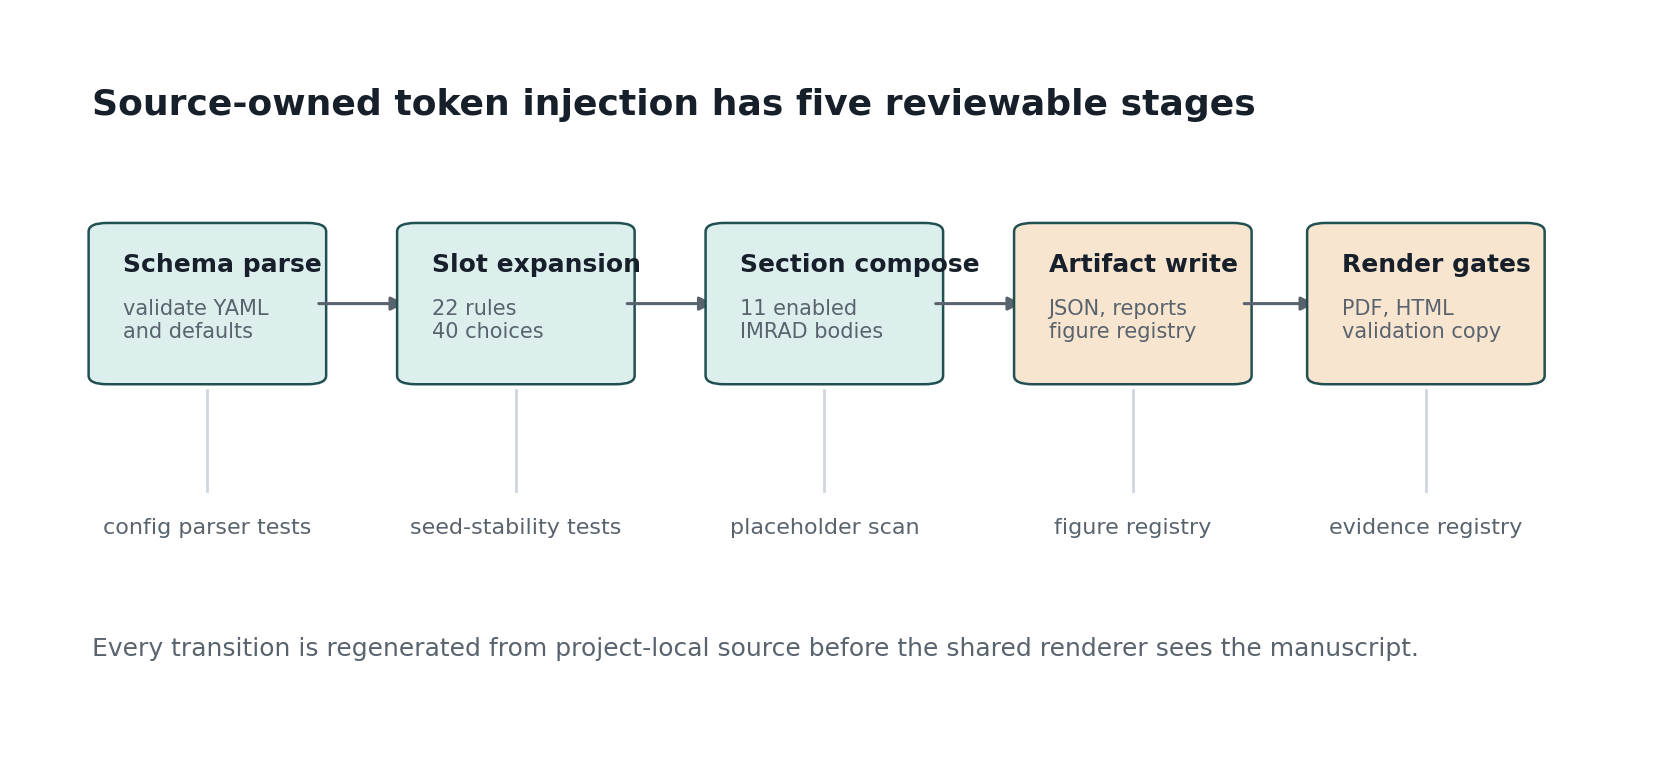
\includegraphics[keepaspectratio,alt={Deterministic token-injection flow}]{../figures/token_injection_flow.png}}
\caption{Deterministic token-injection
flow}\label{fig:token-injection-flow}
\end{figure}
\end{frame}

\begin{frame}[allowframebreaks]{Design Principles}
\protect\phantomsection\label{design-principles}
{\def\LTcaptype{none} % do not increment counter
\begin{longtable}[]{@{}
  >{\raggedright\arraybackslash}p{(\linewidth - 4\tabcolsep) * \real{0.3333}}
  >{\raggedright\arraybackslash}p{(\linewidth - 4\tabcolsep) * \real{0.3333}}
  >{\raggedright\arraybackslash}p{(\linewidth - 4\tabcolsep) * \real{0.3333}}@{}}
\toprule\noalign{}
\begin{minipage}[b]{\linewidth}\raggedright
Principle
\end{minipage} & \begin{minipage}[b]{\linewidth}\raggedright
Rationale
\end{minipage} & \begin{minipage}[b]{\linewidth}\raggedright
Manuscript effect
\end{minipage} \\
\midrule\noalign{}
\endhead
Configuration owns prose choices & Reviewers can inspect the declared
language surface before generation. & Large-grain manuscript variables
are generated from YAML and project source. \\
Method surface is config-owned & A fork should change method protocol
rows before changing generated Methods prose. & The Methods tables and
body summarize method\_protocol and pipeline\_phases from YAML. \\
Token choice is deterministic & A fixed seed and lexicon must produce
the same injection plan across reruns. & Token inventory rows can be
regenerated and diffed. \\
Field origin is evidence & A generated manuscript should distinguish
authored YAML fields from loader defaults. & Configured-field tables and
figures report explicit and defaulted paths. \\
Sections are conditional but visible & Disabled material should be
auditable rather than silently absent. & Every disabled section resolves
to an explicit disabled-section body. \\
Visual audit follows data & Figures should explain the generated method
without becoming decorative claims. & Cover, flow, allocation,
provenance, gate, and field-origin figures are regenerated from
artifacts. \\
Generated output is disposable & The durable artifact is the
regeneration contract, not hand-edited output files. & Output Markdown,
PDF, HTML, and slides are rebuilt from source inputs. \\
Claim boundaries travel with prose & Generated text can otherwise imply
validation that no artifact supports. & Contribution, limitation,
failure-mode, and authoring tables carry boundary text. \\
Forks must add validators & Domain claims need domain evidence beyond
this exemplar's generic regeneration gates. & Scope, limitations, and
authoring contract require validators before domain claims. \\
Invariants precede rendering & Readers need to know which inputs are
allowed to alter generated tokens before they inspect output. & Methods
names the digest inputs and excludes renderer state from token
choice. \\
Diffs are review objects & Config, token inventory, manuscript
variables, figures, and copied outputs should be diffable review
surfaces. & Methods and reproducibility text describe review packet
assembly after regeneration. \\
Review packet is a method artifact & A PDF alone is insufficient
evidence for a generated-method exemplar. & Authoring contract and
validation sections treat data, reports, figures, and logs as part of
review. \\
Fork migration is part of the method & A public exemplar should teach
authors what must change before domain use. & Standalone notes,
authoring obligations, and claim-ledger boundaries name fork
responsibilities. \\
\bottomrule\noalign{}
\end{longtable}
}
\end{frame}

\begin{frame}[fragile,allowframebreaks]{Operational Phases}
\protect\phantomsection\label{operational-phases}
{\def\LTcaptype{none} % do not increment counter
\begin{longtable}[]{@{}
  >{\raggedright\arraybackslash}p{(\linewidth - 8\tabcolsep) * \real{0.2000}}
  >{\raggedright\arraybackslash}p{(\linewidth - 8\tabcolsep) * \real{0.2000}}
  >{\raggedright\arraybackslash}p{(\linewidth - 8\tabcolsep) * \real{0.2000}}
  >{\raggedright\arraybackslash}p{(\linewidth - 8\tabcolsep) * \real{0.2000}}
  >{\raggedright\arraybackslash}p{(\linewidth - 8\tabcolsep) * \real{0.2000}}@{}}
\toprule\noalign{}
\begin{minipage}[b]{\linewidth}\raggedright
Phase
\end{minipage} & \begin{minipage}[b]{\linewidth}\raggedright
Input
\end{minipage} & \begin{minipage}[b]{\linewidth}\raggedright
Transformation
\end{minipage} & \begin{minipage}[b]{\linewidth}\raggedright
Output
\end{minipage} & \begin{minipage}[b]{\linewidth}\raggedright
Guard
\end{minipage} \\
\midrule\noalign{}
\endhead
Schema intake & \breaktt{manuscript/config.yaml} & Load paper metadata
and validate the madlib schema before generation. &
\texttt{MadlibConfig} & config parser tests \\
Scenario declaration & \texttt{MadlibConfig} & Summarize local scope,
enabled sections, claim boundaries, and review handoff expectations. &
\breaktt{review\ scenario} & method protocol and contribution table
tests \\
Field-origin inventory & \breaktt{MadlibConfig\ and\ raw\ YAML\ keys} &
Classify supported paths as explicit or defaulted. &
\breaktt{configured\_field\_inventory.json} & configured-field inventory
tests \\
Lexicon validation & \breaktt{madlib.lexicon\ and\ madlib.slots} & Reject
empty required categories and slot references to missing categories. &
\breaktt{validated\ slot\ inventory} & malformed-config tests \\
Digest token planning & \texttt{MadlibConfig} & Hash seed, slot name,
category, ordinal, and category inventory. & \texttt{TokenPlan} &
seed-stability tests \\
Invariant review & \breaktt{TokenPlan\ and\ method\ protocol} & Confirm
allowed token-choice inputs are documented and isolated from renderer
state. & \breaktt{selection\ invariant\ set} & token determinism and
Methods prose tests \\
Slot-to-section allocation & \texttt{TokenPlan} & Assign each selected
token to its configured manuscript section. &
\breaktt{section\ token\ counts} & provenance and allocation tests \\
Section composition & \breaktt{TokenPlan\ and\ narrative\ moves} & Build
conditional section bodies, titles, and evidence tables. &
\breaktt{manuscript\ variable\ map} & placeholder-coverage tests \\
Evidence table assembly & \breaktt{MadlibConfig\ and\ TokenPlan} & Render
protocol, phase, audit, token, section, provenance, and configured-field
tables. & \breaktt{manuscript\_variables.json} & composition table
tests \\
Claim-ledger alignment &
\breaktt{MadlibConfig,\ generated\ prose,\ and\ data/claim\_ledger.yaml}
& Check local claims and non-claims against source-owned evidence rows.
& \breaktt{claim-aligned\ evidence\ surface} & claim ledger and evidence
registry review \\
Visualization emission &
\breaktt{MadlibConfig,\ TokenPlan,\ and\ configured-field\ inventory} &
Generate cover, flow, allocation, provenance, gate, and configured-field
figures. & \breaktt{output/figures\ and\ figure\_registry.json} &
nonblank figure tests \\
Artifact emission & \breaktt{MadlibConfig\ and\ TokenPlan} & Write
inventory, section plan, injection trace, summary, cover overview,
manuscript figures, and registry. &
\breaktt{output/data,\ output/reports,\ and\ output/figures} &
artifact-writing tests \\
Manuscript hydration &
\breaktt{source\ manuscript\ shells\ and\ manuscript\_variables.json} &
Resolve large-grain placeholders into output/manuscript. &
\breaktt{hydrated\ Markdown\ manuscript} & unresolved-token scan \\
Render & \breaktt{output/manuscript} & Render PDF, HTML, and slides
through the shared template pipeline. &
\breaktt{output/pdf,\ output/web,\ and\ output/slides} & render
command \\
Validate and copy & \breaktt{project\ output\ directories} & Validate
files, registries, evidence, overlays, and copied deliverables. &
\breaktt{output/templates/template\_madlib} & validation and copy
commands \\
Review packet assembly &
\breaktt{validated\ project\ output\ and\ copy\ statistics} & Group
manuscript, web, slides, figures, data, reports, validation results, and
copy statistics as the review surface. & \texttt{review\ packet} &
copied-output validation \\
Fork contract documentation &
\breaktt{source\ docs,\ authoring\ contract,\ and\ claim\ ledger} & State
which config, source, test, validator, and evidence surfaces a fork must
change before domain claims. & \breaktt{fork\ migration\ notes} &
documentation and claim-ledger tests \\
\bottomrule\noalign{}
\end{longtable}
}
\end{frame}

\begin{frame}[fragile,allowframebreaks]{Protocol Steps}
\protect\phantomsection\label{protocol-steps}
{\def\LTcaptype{none} % do not increment counter
\begin{longtable}[]{@{}
  >{\raggedright\arraybackslash}p{(\linewidth - 6\tabcolsep) * \real{0.2500}}
  >{\raggedright\arraybackslash}p{(\linewidth - 6\tabcolsep) * \real{0.2500}}
  >{\raggedright\arraybackslash}p{(\linewidth - 6\tabcolsep) * \real{0.2500}}
  >{\raggedright\arraybackslash}p{(\linewidth - 6\tabcolsep) * \real{0.2500}}@{}}
\toprule\noalign{}
\begin{minipage}[b]{\linewidth}\raggedright
Step
\end{minipage} & \begin{minipage}[b]{\linewidth}\raggedright
Action
\end{minipage} & \begin{minipage}[b]{\linewidth}\raggedright
Evidence
\end{minipage} & \begin{minipage}[b]{\linewidth}\raggedright
Output
\end{minipage} \\
\midrule\noalign{}
\endhead
Ingest declared manuscript schema & Parse paper metadata and the madlib
block from manuscript/config.yaml before any prose or figures are
composed. & Config validation tests and MadlibConfig construction from
the committed YAML. & \texttt{MadlibConfig} \\
Declare review scenario & Name the manuscript scope, local claim
boundary, enabled sections, and intended reviewer handoff before token
generation. & section\_plan.json, contribution table, and authoring
contract rows. & \breaktt{review\ scenario} \\
Track field origin & Record every supported madlib path as explicit when
it appears in YAML or defaulted when the loader supplies it. &
configured\_field\_inventory.json and configured-field origin tests. &
\breaktt{explicit/default\ path\ inventory} \\
Govern lexicon categories & Reject empty required categories, preserve
project-owned optional categories, and treat every lexical list as
source data. & Malformed-config tests and lexicon rows in
token\_inventory.json. & \breaktt{validated\ lexicon} \\
Construct digest selection material & Combine seed, slot name, category,
ordinal, and the full category inventory into a deterministic digest
input. & Seed-stability and category-sensitivity tests. &
\breaktt{digest\ input\ records} \\
Record selection invariants & State the invariant inputs that are
allowed to change token choices and the renderer state that is not
allowed to affect them. & Token determinism tests and Methods digest
prose. & \breaktt{selection\ invariant\ set} \\
Expand slot declarations & Resolve every slot count into one or more
token choices and assign each selected value to its configured
manuscript section. & TokenPlan construction, provenance trace, and
section allocation figure. & \texttt{TokenPlan} \\
Apply section conditions & Evaluate section switches before prose
assembly so disabled sections receive explicit disabled-section bodies.
& Section-condition tests and output/data/section\_plan.json. &
\breaktt{enabled\ section\ set} \\
Compose conditional IMRAD bodies & Build large-grain section variables
from narrative moves, selected tokens, section switches, and local claim
boundaries. & Generated manuscript variables and hydrated
output/manuscript Markdown. & \breaktt{section\ variables} \\
Assemble evidence tables & Render method protocol, pipeline phase,
design principle, audit rule, token inventory, section plan, and
provenance tables from config and TokenPlan. & Composition tests and
generated manuscript\_variables.json table entries. &
\breaktt{Markdown\ evidence\ tables} \\
Align claims with evidence ledger & Keep generated method,
visualization, and publication-boundary claims tied to config, source
modules, generated artifacts, or explicit non-claim boundaries. &
data/claim\_ledger.yaml and evidence registry validation. &
\breaktt{claim-aligned\ evidence\ surface} \\
Generate visual audit surface & Write the cover overview,
token-injection flow, section allocation, provenance trace, quality
gate, and configured-field figures from generated data. & Nonblank
figure tests and output/figures/figure\_registry.json. &
\breaktt{registered\ figure\ set} \\
Emit machine-readable artifacts & Write token inventory, section plan,
configured-field inventory, injection trace, summary reports, validation
inputs, and figure registry. & Artifact-writing tests, artifact
manifest, and validation reports. &
\breaktt{output/data,\ output/reports,\ and\ output/figures} \\
Hydrate manuscript shell & Write manuscript\_variables.json and resolve
the source Markdown shells into output/manuscript. & Unresolved-token
scan and render validation. & \breaktt{output/manuscript} \\
Render and validate deliverables & Render PDF, HTML, and slides through
shared infrastructure, then validate PDFs, Markdown, figure registry,
evidence registry, design overlays, and artifact manifest. & Stage 03
render log and Stage 04 validation report. &
\breaktt{validated\ project\ output} \\
Assemble reviewer packet & Treat hydrated Markdown, rendered PDF, web
output, slides, figures, data, reports, validation logs, and copied
output statistics as one review packet. & Stage 04 validation report and
Stage 05 output\_statistics.json. & \texttt{review\ packet} \\
Copy review surface & Copy validated deliverables into
output/templates/template\_madlib only after validation passes. & Stage
05 copy statistics and copied-output validation. &
\breaktt{copied\ publication-review\ bundle} \\
Document fork migration & Record what downstream authors must change
when moving from exemplar token injection to a domain-specific report. &
README, STANDALONE notes, manuscript README, Authoring Contract, and
claim ledger boundary rows. & \breaktt{fork\ migration\ notes} \\
\bottomrule\noalign{}
\end{longtable}
}
\end{frame}

\begin{frame}[allowframebreaks]{Section Plan}
\protect\phantomsection\label{section-plan}
{\def\LTcaptype{none} % do not increment counter
\begin{longtable}[]{@{}
  >{\raggedright\arraybackslash}p{(\linewidth - 8\tabcolsep) * \real{0.1765}}
  >{\raggedright\arraybackslash}p{(\linewidth - 8\tabcolsep) * \real{0.1765}}
  >{\raggedleft\arraybackslash}p{(\linewidth - 8\tabcolsep) * \real{0.2353}}
  >{\raggedleft\arraybackslash}p{(\linewidth - 8\tabcolsep) * \real{0.2353}}
  >{\raggedright\arraybackslash}p{(\linewidth - 8\tabcolsep) * \real{0.1765}}@{}}
\toprule\noalign{}
\begin{minipage}[b]{\linewidth}\raggedright
Section
\end{minipage} & \begin{minipage}[b]{\linewidth}\raggedright
Render title
\end{minipage} & \begin{minipage}[b]{\linewidth}\raggedleft
Enabled
\end{minipage} & \begin{minipage}[b]{\linewidth}\raggedleft
Token choices
\end{minipage} & \begin{minipage}[b]{\linewidth}\raggedright
Narrative moves
\end{minipage} \\
\midrule\noalign{}
\endhead
abstract & Abstract & True & 3 & state the manuscript-generation
problem, name the deterministic intervention, summarize the audit
surface \\
introduction & Introduction: Lexicon as Data and Manuscript as Build
Artifact & True & 8 & separate playful Mad Lib syntax from research
claims, identify drift between prose and source data, frame
configuration as an inspectable dataset, position conditional prose as a
reproducibility problem \\
methods & Methods: Source-Owned Token Injection and Conditional IMRAD
Assembly & True & 6 & validate config before composition, declare review
scenario and method invariants, separate explicit YAML fields from
loader defaults, govern lexicon categories as reviewable data, expand
slots through seeded digest selection, allocate slot choices to enabled
manuscript sections, compose conditional section bodies, assemble method
evidence tables and visual audit figures, align generated claims with
the claim ledger, emit evidence artifacts before rendering, verify that
no unresolved placeholders remain, assemble a reviewer packet from
regenerated artifacts, preserve human review before publication
claims \\
results & Results: Provenance, Density, and Resolved Manuscript Surface
& True & 5 & report token density, show resolved section coverage, bind
every manuscript token to provenance, connect the figure and inventory
to the same plan \\
discussion & Discussion: Accountability Boundaries for Generated Prose &
True & 3 & bound the scholarly claim, describe useful adaptation cases,
name misuse modes, preserve human authorship responsibility \\
configuration & Configuration: Schema-Controlled Lexicon, Slots, and
Narrative Moves & True & 1 & document schema ownership, show title and
switch behavior, record generated counts from code \\
evaluation & Evaluation: Gate Criteria, QA Probes, and Failure Discovery
& True & 5 & name readiness criteria, connect criteria to artifacts,
separate local checks from publication readiness, make failure probes
visible \\
reproducibility & Reproducibility: Seeded Regeneration and Artifact
Trace & True & 2 & fix seed and config hash, write machine-readable
artifacts, rerender through the shared pipeline, copy outputs only after
validation \\
limitations & Limitations: Non-Claims, Misuse Modes, and Human Review &
True & 3 & state non-claims, identify misuse modes, preserve human
review, require domain validators for domain claims \\
scope & Scope: Related Generators and Responsible Forking & True & 2 &
distinguish generation from truth, limit publication claims, point to
local evidence, explain responsible forking \\
authoring\_contract & Authoring Contract: Human Review and Forking
Obligations & True & 2 & state human responsibilities, name fork
obligations, connect review to generated evidence, require domain
validators before domain claims, document fork migration notes \\
\bottomrule\noalign{}
\end{longtable}
}
\end{frame}

\begin{frame}[allowframebreaks]{Audit Rules}
\protect\phantomsection\label{audit-rules}
{\def\LTcaptype{none} % do not increment counter
\begin{longtable}[]{@{}
  >{\raggedright\arraybackslash}p{(\linewidth - 2\tabcolsep) * \real{0.5000}}
  >{\raggedright\arraybackslash}p{(\linewidth - 2\tabcolsep) * \real{0.5000}}@{}}
\toprule\noalign{}
\begin{minipage}[b]{\linewidth}\raggedright
Rule
\end{minipage} & \begin{minipage}[b]{\linewidth}\raggedright
Enforcement surface
\end{minipage} \\
\midrule\noalign{}
\endhead
R1 & Every manuscript placeholder must be generated by source code. \\
R2 & Every generated token choice must carry category and config-key
provenance. \\
R3 & Every method protocol row must identify an action, evidence
artifact, and output. \\
R4 & Every pipeline phase must identify an input, transformation,
output, and guard. \\
R5 & Every visible configured field must be classified as explicit or
defaulted. \\
R6 & Every disabled section must resolve to an explicit disabled-section
body. \\
R7 & Every figure reference must be backed by a generated figure
registry entry. \\
R8 & Every fork that adds domain claims must add domain validators and
claim-ledger evidence. \\
R9 & Every publication claim must stay local unless a live DOI or
release exists. \\
R10 & Every token-selection explanation must name only seed, slot,
category, ordinal, and ordered category inventory as digest inputs. \\
R11 & Every review handoff must include generated data, reports,
figures, validation results, and copy statistics alongside PDF or
HTML. \\
R12 & Every fork migration note must name config, source, test,
validator, pipeline, and claim-ledger obligations. \\
\bottomrule\noalign{}
\end{longtable}
}
\end{frame}

\end{document}
